\chapter{Experimental Setup and Results}

In this chapter, I will describe our experimental setup and results. It includes a brief discussion of our optical tables setup (\ref{exp:laser-table} and \ref{exp:machine-table}), the implementation, optimization and performance of each steps (\ref{exp:mot}, \ref{exp:gm}, \ref{exp:pump}, \ref{exp:mt} and \ref{exp:odt}) and finally some basic characteristic of our BEC (\ref{exp:odt}). The discussion will fucuses mainly on the main coil configuration (\ref{exp:coil}), gray molasses alignment (\ref{exp:gm}) and stray field zeroing for the quadrupole magnetic trap \ref{exp:mt} in which I had the most contribution.\\
\\
The other important parts of the experiment are going to be discussed briefly in order to give a complete picture of the experiment. A more detailed description of some part of the experiment, especially the vacuum system, the laser system, the optimization of the RF evapration in the magnetic trap, the optical dipole trap and the BEC, are expected to be found in the PhD thesis of the current senior graduate students.

\section{Laser System}\label{exp:laser-table}
The laser table is where we prepare all the light sources used in the experiment that is closed to resonance with the Lithium-$7$ $D1$ and $D2$ lines. In this section, I will give a description of our laser system. Instead of going into technical details about the setup, which will be included in one of the future PhD thesis, I am going to briefly describe the goal of the system, the techniques we use, and the performance of it.\\
\\
As discussed in the theoretical chapter, we need mainly four different frequency ranges for the laser cooling and manipulation of the atoms. For the Zeeman slower and MOT, we need the $D2$ line (\ref{theory:mot}) and we use the $D1$ line for the gray molasses (\ref{theory:gm}). For the dark state pumping that will be discussed later (\ref{exp:pump}), we also use the $D1$ line. Furthermore, in all of these cases, we also need two frequencies to address the atoms in both of the hyperfine ground states $F=1$ and $F=2$, which are conveniently called $F1$ and $F2$ light. The goal of the laser table is therefore generating these four different frequencies ranges and deliver them to the machine table using optical fibers.\\
\\
Since the separation between $D1$ and $D2$ is larger than most of the common optical frequency shifters (e.g. AOMs), we generate the $D1$ and $D2$ light by locking two diode lasers on to the appropriate atomic transition using saturated absorption spectroscopy. Since we do not need $D1$ and $D2$ light at the same time, we use an AOM in each of the $D1$ and $D2$ beam path to swich the light and determine which frequency goes to the rest of the system. In the $D2$ path, we also use a $300MHz$ AOM in the double pass setup to get the right frequency for the Zeeman slower.\\
\\
After getting one of the $D$ line we want, we use a $50$-$50$ cube beam splitter to put them into the $F1$ and $F2$ path. Since the hyperfine splitting of the ground state for Lithium-$7$ is relatively small ($803.5MHz$), we use a $400MHz$ AOM in the double pass setup to blue shift the frequency from $F2$ to $F1$ and to fine tune the frequency in certain range. For the $F2$ pass, two AOM's in the tandem setup are used for frequency fine tuning.\\
\\
The frequency generation stage is followed by an amplification stage using one tapered amplifier per-path to generate the power we want. After that we use AOM's, shutters and other optics to switch the laser, couple them into the fibers with the right polarization and deliver them to the machine table where we use them to manipulate the atoms.

\section{Vacuum Chamber and Main Coils Configuration}\label{exp:machine-table}

In this section, I am going to describe some important setup on the machine table where out vacuum chamber sits on.

\subsection{Optical Access of the Vacuum Chamber}\label{exp:chamber}
\begin{figure}
  \begin{center}
    \begin{tikzpicture}[scale=0.8]
      % ODT windows
      \draw[rotate around={22.5:(0, 0)},line width=2] (-4.3, -.35) rectangle (4, .35);
      \draw[rotate around={-22.5:(0, 0)},line width=2] (-4.3, -.35) rectangle (4, .35);

      % MOT windows
      \draw[rotate around={45:(0, 0)},line width=2] (-3.2, -.7) rectangle (3.2, .7);
      \draw[rotate around={-45:(0, 0)},line width=2] (-3.2, -.7) rectangle (3.2, .7);

      % Slower windows
      \draw[line width=2] (0, -.8) rectangle (3.2, .8);
      \draw[line width=2] (-4, -.3) rectangle (0, .3);

      % Imaging windows
      \draw[line width=2] (-1.2, 0) rectangle (1.2, 3.2);
      \draw[line width=2] (-.4, 0) rectangle (.4, -3.2);

      % Main Chamber
      \draw[fill=white,line width=2] (0, 0) circle (3);

      % Coils
      \draw[line width=1,fill=brown] (0, 0) circle (2.5);
      \draw[line width=1] (0, 0) circle (2.3);
      \draw[line width=1] (0, 0) circle (2.1);
      \draw[line width=1] (0, 0) circle (1.9);
      \draw[line width=1] (0, 0) circle (1.7);
      \draw[line width=1,fill=white] (0, 0) circle (1.5);
      \path (0, 2) node[align=center,white] {\textbf{Main}\\\textbf{Coils}};

      % MOT beams
      \draw[line width=2,snake arrow,rotate around={45:(0, 0)},red] (6, 0) node[right] {MOT/GM} -- ++(-2.5, 0);
      \draw[line width=2,snake arrow,rotate around={-45:(0, 0)},red] (6, 0) node[right] {MOT/GM} -- ++(-2.5, 0);
      \draw[line width=2,snake arrow,rotate around={135:(0, 0)},red] (6, 0) node[right] {MOT/GM} -- ++(-2.5, 0);
      \draw[line width=2,snake arrow,rotate around={-135:(0, 0)},red] (6, 0) node[right] {MOT/GM} -- ++(-2.5, 0);

      % Imaging
      \draw[line width=1,snake arrow,rotate around={-90:(0, 0)},red] (6, 0) node[right,align=center] {Imaging/\\Dark State Pumping} -- ++(-2.5, 0);

      % ODT1
      \draw[line width=4,snake arrow,rotate around={22.5:(0, 0)}] (6, 0) node[right] {ODT} -- ++(-2, 0);
      \draw[line width=.5,snake arrow,rotate around={22.5:(0, 0)},red] (6, -0.2) -- ++(-2, 0);
      \path[rotate around={22.5:(0, 0)},red] (5, 0) node[below right,align=center] {Side\\Imaging};

      % ODT2
      \draw[line width=4,snake arrow,rotate around={-22.5:(0, 0)}] (6, 0) node[right] {ODT} -- ++(-2, 0);
      \draw[line width=.5,snake arrow,rotate around={-22.5:(0, 0)},red] (6, 0.2) -- ++(-2, 0);
      \path[rotate around={-22.5:(0, 0)},red] (5, 0) node[above right,align=center] {Side\\Imaging};
      \draw[line width=3,snake arrow,rotate around={-22.5:(0, 0)},green] (6, -0.3) -- ++(-2, 0);
      \path[rotate around={-22.5:(0, 0)},green] (5, -0.3) node[below left] {Plug};

      % Slower
      \draw[line width=2,snake arrow,red] (6, 0) node[right,align=center] {Zeeman\\Slower} -- ++(-2.5, 0);
      \draw[line width=4,->,rotate around={180:(0, 0)}] (6, 0) node[left,align=center] {Atoms\\From Oven} -- ++(-2, 0);
    \end{tikzpicture}
  \end{center}
  \caption{Top View of the Vacuum Chamber (Top/Bottom MOT/Gray Molasses beams not included, not to scale).}
  \label{chamber-light}
\end{figure}
The windows and connections except the top and bottom window on our main vacuum chamber is shown in figure \ref{chamber-light}. There are in total $6$ MOT/Gray Molasses beams, $2$ ODT beams, $3$ Imaging beams, a plug and a Zeeman slower beam going into the chamber. When multiple colors need to be sent in through the same window, they are combined outside the vacuum chamber using appropriate dichroic.

\subsection{MOT-Gray Molasses Cage}\label{exp:mot-cage}
\begin{figure}
  \begin{center}
    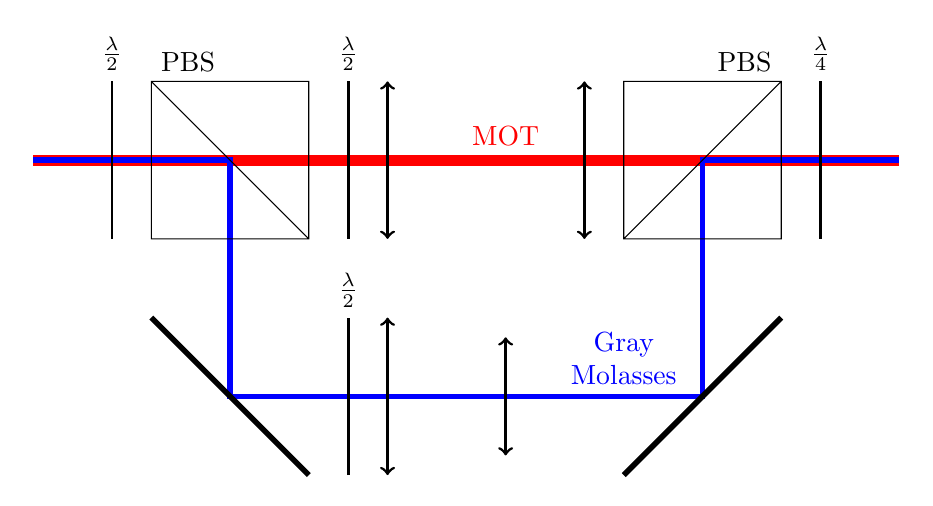
\begin{tikzpicture}
      \draw[line width=4,red] (-1, 1) -- (5, 1) node[above] {MOT} -- (10, 1);

      \draw[line width=2,blue] (-1, 1) -- (1.5, 1) -- ++(0, -3) -- (6.5, -2) node[above,align=center] {Gray\\Molasses} -- (7.5, -2) -- (7.5, 1) -- (10, 1);

      \draw[line width=1] (0, 0) -- ++(0, 2) node[above] {$\frac{\lambda}{2}$};
      \draw (0.5, 2) rectangle ++(2, -2) -- ++(-2, 2) node[above right] {PBS};
      \draw[line width=1] (3, 0) -- ++(0, 2) node[above] {$\frac{\lambda}{2}$};
      \draw[line width=1,<->] (3.5, 0) -- ++(0, 2);
      \draw[line width=1,<->] (6, 0) -- ++(0, 2);
      \draw (6.5, 0) rectangle ++(2, 2) node[above left] {PBS} -- ++(-2, -2);
      \draw[line width=1] (9, 0) -- ++(0, 2) node[above] {$\frac{\lambda}{4}$};

      \draw[line width=2] (2.5, -3) -- ++(-2, 2);
      \draw[line width=1] (3, -3) -- ++(0, 2) node[above] {$\frac{\lambda}{2}$};
      \draw[line width=1,<->] (3.5, -3) -- ++(0, 2);
      \draw[line width=1,<->] (5, -2.75) -- ++(0, 1.5);
      \draw[line width=2] (8.5, -1) -- ++(-2, -2);
    \end{tikzpicture}
  \end{center}
  \caption{MOT/Gray Molasses Cage.}
  \label{mot-cage-design}
\end{figure}
The delivery of the MOT and gray molasses beam from the two in-coupler on the laser table to the six output on the machine table is done with a polarization maintaining evanescent wave fiber splitter which takes the light from the two input fibers and split them equally into the six output fibers. However, the MOT beams and the gray molasses beams have different requirement in beam sizes. On one hand, the MOT needs a bigger beam size for a bigger capture volume. On the other hand, as discussed earlier, for the gray molasses to work effectively, high intensity, therefore smaller beam size, is required. In order to have a different size for the two beams coming out of the same fiber, we send in the two beams with orthogonal polarization's and add polarization dependent beam expenders after the fiber output to shape the two beams differently. This beam shaping is done with a cage system shown in figure \ref{mot-cage-design}. The upper beam path is used for expanding the MOT beam whereas the lower path shapes the gray molasses beam to a smaller size. Each of the four lenses can slide in the cage, which are used to tweak the size and divergence of the beams. The alignment between beams is done with the two bottom mirrors and the two half wave-plates between the two polarization beam splitter cubes are used to balance the intensities.

\subsection{Main Coils Configuration}\label{exp:coil}
\begin{figure}
  \begin{center}
    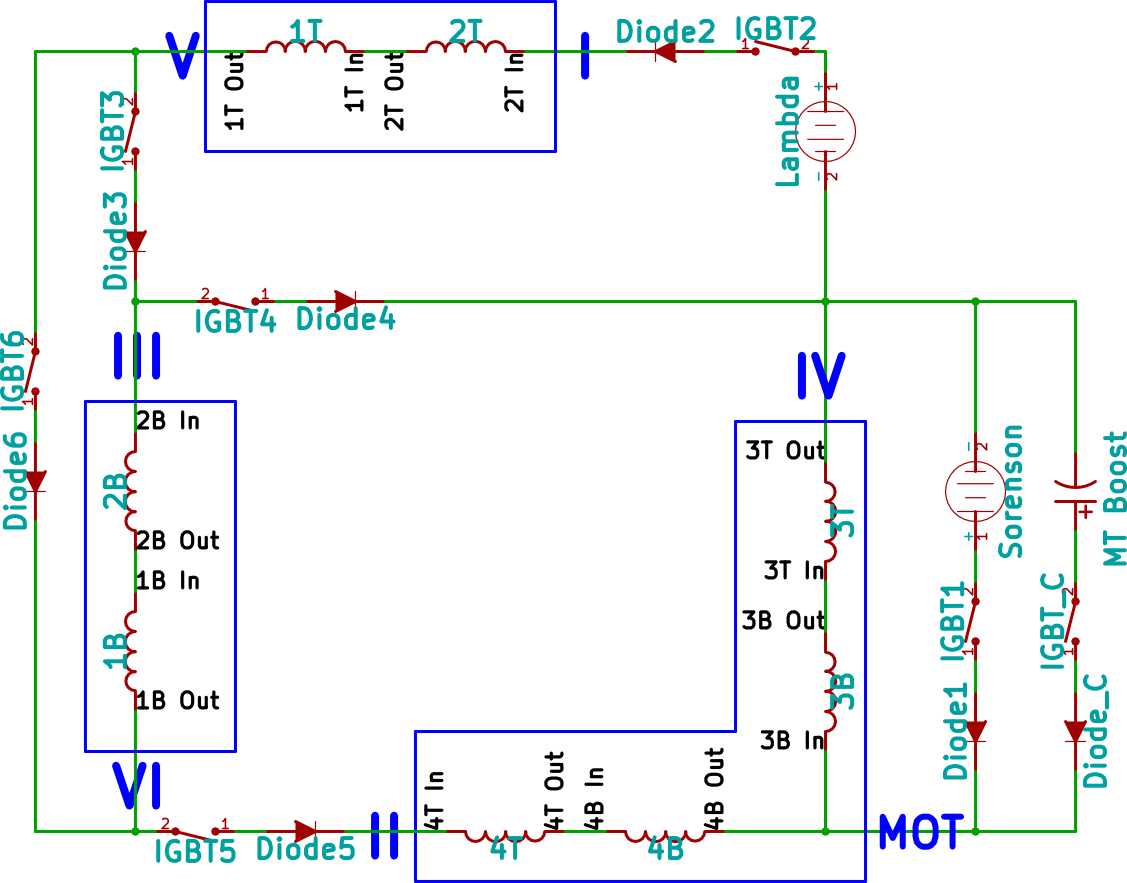
\includegraphics[width=15cm]{coil.png}
  \end{center}
  \caption{Main Coils Control Circuit. (Magnetic trap boost capacitor charging circuit not included.)}
  \label{exp:coil-control}
\end{figure}
\begin{table}
  \begin{center}
    \begin{tabular}{|c|c|c|}\hline
      \multirow{2}{*}{Closed switches(IGBTs)}& \multicolumn{2}{c|}{Usage of the power supply} \\\hhline{~--}
      &Lambda&Sorenson\\\hline
      1, 3, 5&-&\begin{tabular}{@{}c@{}}Quadrupole field with\\layer 3 for MOT and ODT\\clean up (\ref{exp:odt})\end{tabular}\\\hline
      2, 3, 5&\begin{tabular}{@{}c@{}}Quadrupole field with\\layer 1, 2, 3 and 4 for\\magnetic trap\end{tabular}&-\\\hline
      1, 2, 4, 6&\begin{tabular}{@{}c@{}}Homogeneous Feshbach resonance\\field with layer 1 and 2\end{tabular}&\begin{tabular}{@{}c@{}}Field gradient on top of\\the bias field with layer 3\\for tilt and levitation.\end{tabular}\\\hline
    \end{tabular}
  \end{center}
  \caption{List of coil configurations}
  \label{exp:coil-config}
\end{table}
Besides the weak field (up to several Gauss) provided by the shim coils for earth field compensation and small bias field, we use strong magnetic field in the experiment in many different configurations. In the magneto-optical trap, we need a quadrupole field ($\approx20\text{G}\cdot\text{cm}^{-1}$). For the static magnetic trap, we use a stronger quadrupole field ($\approx500\text{G}\cdot\text{cm}^{-1}$). And finally for the evaporation in the optical dipole trap, we need independent control of a very strong bias field (up to $\approx1000\text{G}$) and a gradient on top of it (up to $\approx30\text{G}\cdot\text{cm}^{-1}$). In order to avoid interference between different steps of the experiment, we also need the capability of turning on and off or changing the configuration of the magnetic field quickly ($\ll1\text{ms}$).\\
\\
These strong magnetic field is generated in the experiment by running up to $500\text{A}$ of current through one pair of water cooled coils attached to the vacuum chamber. The coils are positioned closed to the Helmholtz condition to maximize the homogeneity when generating a bias field. Each of the coil consists of $5$ layers which can be connected and powered independently (one of them is damaged during operation and is not used currently) so that they can be used in different configurations. Due to the limitation of our power supplies (both in output capability and in the number we have), many of the field configuration we need requires running current through more than one layer of the coils. Therefore, in order to achieve different configuration of the field, it is necessary to reuse our power supplies and coil layers in different steps.\\
\\
The options available for fast switching of such high current are mechanical relays or solid state (semiconductor) devices. After comparing the performance and reliability of different options, we decided to use high power IGBT's (insulated-gate bipolar transistor) since they are the most widely used solid state device for high current application and can provide a lot shorter response time with similar cost and failing rate compare to mechanical relays. The switching time for these IGBT's to switch certain current are determined by the response time of the device (micro-seconds or shorter) and the maximum voltage they can take (since $\ud I/\ud t=L/U$). Since the IGBT's we use can take a voltage higher than $500\text{V}$, simple calculation shows that they can switch off the maximum current we have within $100\mu s$, which is already much shorter than the decay time of the eddy current in our vacuum chamber (mili-second).\\
\\
In order to generate bias field and quadrupole field with our main coil, we can put current into one pair of layers on both side in the same and opposite direction respectively. However, for reusing a layer, we need to switch the polarity of current on one side and keep the direction on the other side the same. Since each IGBT acts like a single throw single pole switch (in one direction), we need four IGBT's (two on each side) to change the polarity of one layer by connecting the two ends of the layer to either side of the supply. This configuration is called a H-bridge. In addition to this, since each of the four switches are closed only in one case, we can put layers in series with one of the switches so that they are only powered in one of the configurations in order to use different number of layers in the two configurations. After considering other factors including geometrical constraint and convenience the modified H-bridge designed we use in our experiment can be seen in figure \ref{exp:coil-control}. ``Lambda'' and ``Sorenson'' are the two power supplies. Each pair of switch and diode represent an IGBT module with floating TTL input control. The layers are numbered as $1T-4T$ and $1B-4B$ meaning the inner layer to side layers on the top and bottom. The ``in'' and ``out'' labels on the layer terminal represent the direction of the current to generate a quadrupole field. Finally, the blue lines separate the parts on the machine table (coils) and the parts on the power supply rack (power supplies and IGBT's) and the blue labels are the connections between the two places. This plot also shows the capacitor (MT Boost) used to boost the magnetic trap turn on with a high voltage. The summary of possible configurations are shown in table \ref{exp:coil-config}.

\section{Magneto-Optical Trap (MOT) and Compressed-MOT}\label{exp:mot}
\begin{figure}
  \begin{center}
    \subfigure[CMOT imaged with $F2$ light.]{
      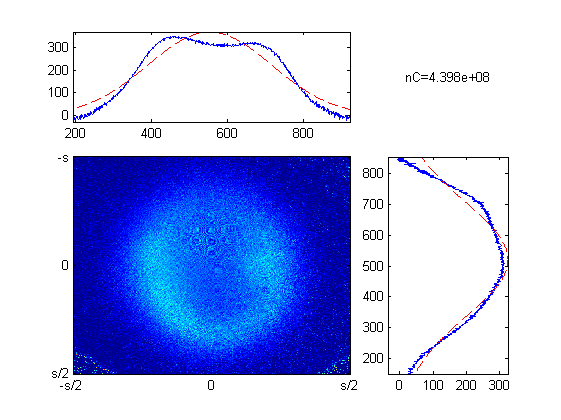
\includegraphics[width=5cm]{cmot-nopump.png}
    }
    \subfigure[CMOT imaged with $F2$ light after pumped into $F2$.]{
      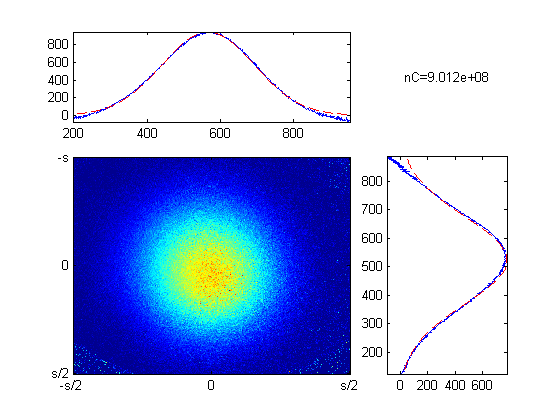
\includegraphics[width=5cm]{cmot-pump.png}
    }
  \end{center}
  \caption{Image of the CMOT. Atoms are pumped into the $F1$ states.}
  \label{exp:cmot-image}
\end{figure}
As the first step of the laser cooling, the MOT loading is optimized by changing the parameters of the lasers to maximize the number of atoms in the MOT after $6$ seconds of loading. The optimum settings we have found are listed in table \ref{exp:mot-param} and the performance of our MOT can be found in table \ref{exp:laser-cooling}.\\
\begin{table}
  \begin{center}
    \begin{tabular}{|c|c|c|c|c|}\hline
      MOT power&Repumper power&MOT detuning&Repumper detuning&MOT Current\\\hline
      $16$mW&$7$mW&$-38.5$mW&$-28$mW&$57$A\\\hline
    \end{tabular}
  \end{center}
  \caption{MOT parameters}
  \label{exp:mot-param}
\end{table}\\
Since our MOT is mainly optimized for loading rate, it is not necessarily optimized for high density and low temperature. Therefore, we added a compress-MOT (CMOT) step after the MOT in order to increase the density and decrease the temperature. In the CMOT step, we ramp the MOT frequency closer to resonance in $4.5$ms and decrease the intensity of the repumper. As a result, the cloud is compressed by radiation pressure and pumped to the $F1$ state. The temperature of the cloud is also decreased because of the decrease in scattering. Figure \ref{exp:cmot-image} shows that the atom in the CMOT are pumped into the $F=1$ states and the performance of the CMOT is listed in table \ref{exp:laser-cooling}.

\section{Gray Molasses}\label{exp:gm}
\begin{figure}
  \begin{center}
    \subfigure[CMOT atoms pumped to $F2$]{
      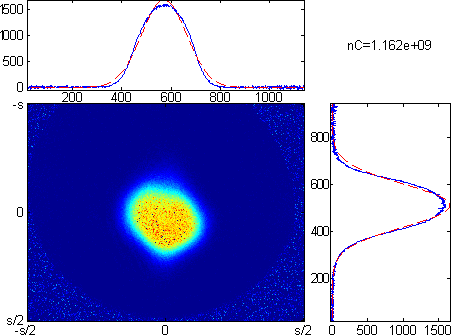
\includegraphics[width=6cm]{gm1-nopump.png}
      \label{exp:gm-align-nopump}
    }
    \subfigure[CMOT atoms pumped to $F2$ and hit with one of the gray molasses beam before alignment]{
      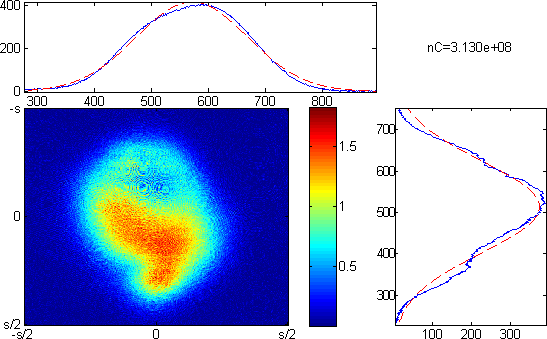
\includegraphics[width=6cm]{gm1-before.png}
      \label{exp:gm-align-before}
    }
    \subfigure[CMOT atoms pumped to $F2$ and hit with one of the gray molasses beam after alignment]{
      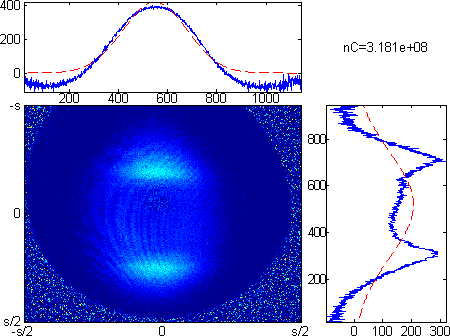
\includegraphics[width=4.5cm]{gm1-after.png}
      \label{exp:gm-align-after}
    }
  \end{center}
  \caption{Images used to align the gray molasses beams.}
  \label{exp:gm-align}
\end{figure}
\begin{figure}
  \begin{center}
    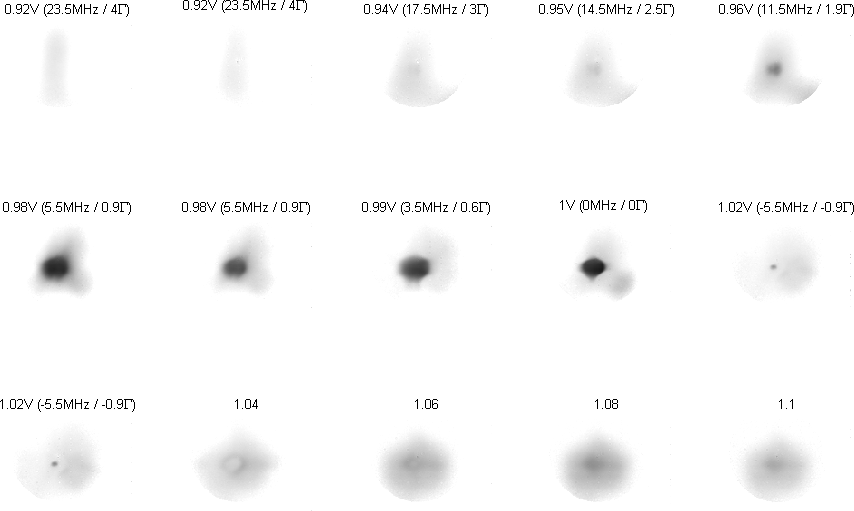
\includegraphics[width=11cm]{gm-ddet.png}
  \end{center}
  \caption{Time of flight image for gray molasses with different relative detuning (in MHz) between the pumper and repumper. (The voltages in the image is the control voltage we use to tweak the frequency.)}
  \label{exp:gm-ddet}
\end{figure}
The gray molasses step is used to cool the CMOT cloud further before transferring to the magnetic trap for evaporative cooling. As mentioned before, we use a smaller size for the gray molasses beam for higher density and better cooling performance. Since the gray molasses only works when the atoms are hit by all of the three pairs of counter-propagating beams, with a gray molasses beam size comparable to that of the cloud after CMOT (both have diameter $\approx5\text{mm}$), one of the challenging tasks for optimizing the gray molasses is to maximize the overlap between the cloud and the six beams while making sure each pairs of the beams are well aligned.\\
\\
Several strategies have been tried to align the gray molasses beams to the desired precision including overlaping with the MOT beams at far field, centering on the window of the vacuum chamber etc. However, since most of these methods relies on the geometry of the machine rather than the atom, we were not able to get the performance we want.\\
\\
In order to overcome this problem, I came up with a method to directly align the beams with the cloud after CMOT to high precision, which can achieve good alignment reliably. The idea is to image the part of the cloud that is missed by each of the beams and to use this image to center the beam on the cloud and minimizing the missing atoms number. In the experiment, this is done by first optically pump all the CMOT atoms into $F=2$ state (figure \ref{exp:gm-align-nopump}) and then shoot the cloud with a short pulse of $F=2$ light from one of the gray molasses beam path while blocking other beams (this is possible without affecting the previous steps because the MOT and gray molasses use different beam paths). Although the atoms hit by the beam will not move so far because of the recoil, the short pulse is enough to pump them into the $F=1$ state. Therefore, imaging with $F=2$ light without a $F=1$ repumper after this will only show the atoms that are not hit by the beam. Figure \ref{exp:gm-align-before} shows one of these images for a the gray molasses beam after aligning only with the center of the chamber, in which we can clearly see shells of atoms missed by the beam. After aligning the beam with the cloud using this image, we got an image of the missing part which looks like \ref{exp:gm-align-after}. We then repeat this procedure on all the beams as well as overlaping each pair of counter-propagating beams to make sure the gray molasses is well aligned with the CMOT cloud.\\
\\
After we repeated this on all the gray molasses beams, we took time of flight images while scanning the frequencies of the light. As shown in figure \ref{exp:gm-ddet}, a clear decrease in temperature (a decrease in time of flight size) can be seen just as what we expected from the theory\ref{theory:gm} and the experimental result from other groups\cite{gm-theory}. The final performance of the gray molasses is also listed in table \ref{exp:laser-cooling}. Since the gray molasses step provide not spacial confinement, being able to maintain the same density as shown in the table confirms that the gray molasses is effecient enough to significantly cool the atoms before they fly away.
\begin{table}
  \begin{center}
    \begin{tabular}{|c|c|c|c|c|}\hline
      Step&Atom Numbers&Temperature(K)&Density($\text{cm}^{-3}$)\\\hline
      Oven&-&$760$&-\\\hline
      Zeeman Slower&-&$0.5$&-\\\hline
      MOT&$2\cdot10^{10}$&$1.5\cdot10^{-3}$&$1\cdot10^{11}$\\\hline
      CMOT&$2\cdot10^{10}$&$1\cdot10^{-3}$&$2\cdot10^{11}$\\\hline
      Gray Molasses&$1\cdot10^{10}$&$1\cdot10^{-4}$&$2\cdot10^{11}$\\\hline
    \end{tabular}
  \end{center}
  \caption{Laser cooling performance.}
  \label{exp:laser-cooling}
\end{table}

\section{Dark State Pumping}\label{exp:pump}
\begin{figure}
  \begin{center}
    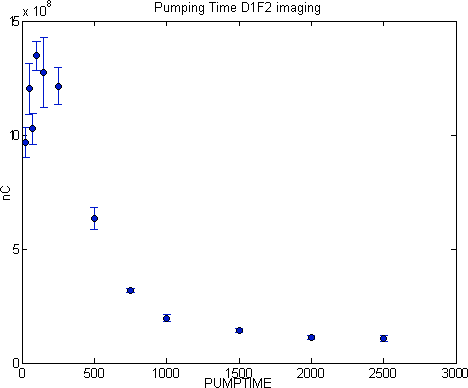
\includegraphics[width=8cm]{mf-pump.png}
  \end{center}
  \caption{Atom number imaged with $D1 (F=2)$ $\sigma^+$ light as a function of dark state pumping time.}
  \label{exp:mf-pump-time}
\end{figure}
At the end of Laser cooling, the atoms are distributed in different hyperfine levels not all of which are trappable. However, in order to transfer to and evaporate in the magnetic trap, all the atoms have to be in a single trappable state. The state we select in our experiment is the $F=2, m_F=2$ state both because it is trappable in any field regime and for a better elastic to inelastic collision rate ratio.\\
\\
For transfering atom into the desired state, we use the technique known as dark state pumping to minimizing the heating from photon scattering during the pumping step. Using the $D1$ transition to the $F'=2$ state, the $F=2, m_F=2$ state is dark for the $\sigma^+$ pumping light. In another word, after the atoms are pumped into the right state, they will become invisible and stop scattering any photons, in contrast with pumping with the $D2$ transition, in which case the atoms in the right state will cycle on the $F=2, m_F=2$ to $F'=3, m_F'=3$ and heats up quickly.\\
\\
Another effect we want to avoid is the re-scattering of the pumping light, which happens when an atom goes into the $F=2$ state and emit a photon close to resonance with the $F=2$ transition with a random polarization that is not necessarily dark for the final state. Since the re-scattering rate is proportional to the scattering rate (i.e. pumping rate) times the scattering cross section, this effect can be minimized by increase the detuning (therefore smaller cross section) and increase the power while keeping a constant scattering rate. With the frequency range we can assess with our apparatus we blue detun the pump light by $\delta_{F1}=20\text{MHz}$ and $\delta_{F2}=34\text{MHz}$ in our experiment for the $F=1$ light and $F=2$ light respectively. Figure \ref{exp:mf-pump-time} shows the atoms after different pumping time imaged with $D1 (F=2)$ $\sigma^+$ light. The initial increase in atom number shows atoms being pumped into $F2$ and the slower decay is when they are going into the $|F=2, m_F=2\rangle$ state invisible to the imaging light.

\section{Magnetic Trap}\label{exp:mt}
\begin{figure}
  \begin{center}
    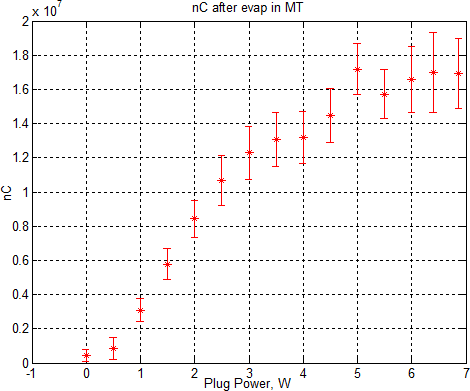
\includegraphics[width=9cm]{plug-power.png}
  \end{center}
  \caption{Saturation of the Plug Laser Power.}
  \label{exp:plug-power}
\end{figure}
\begin{figure}
  \begin{center}
    \subfigure[$x$ direction]{
      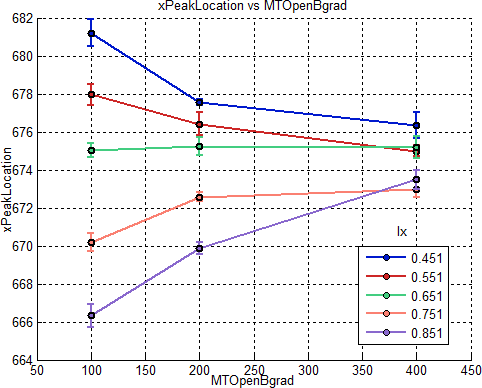
\includegraphics[width=5cm]{field-zeroing-x.png}
    }
    \subfigure[$y$ direction]{
      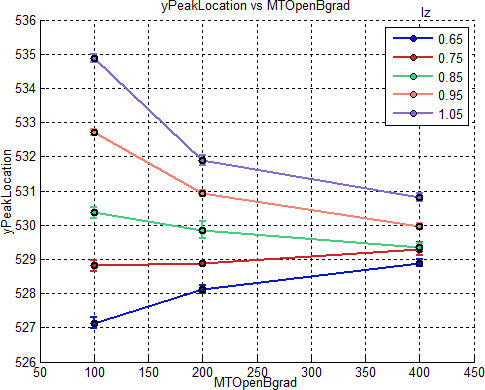
\includegraphics[width=5cm]{field-zeroing-y.png}
    }
  \end{center}
  \caption{Precise Field Zeroing in Magnetic trap}
  \label{exp:field-zeroing}
\end{figure}
In order for an atom to stay trapped in a magnetic trap, it must maintain its Zeeman level. The adiabatic condition, tells us that this means the local magnetic field of an atom should not be too small or change too fast. Although this condition can be easily satisfied for a cold enough cloud, it cannot always hold around the center of the quadrupole magnetic trap where the field goes to zero. Therefore, there is a ``hole'' at the center of a quadrupole trap where atoms can spin flip and escape and the loss caused by this ``hole'' is called Majorana loss. Since the center of the trap is also the lowest point of the trapping potential and therefore is where the atom density is maximized, we will see large Majorana lossing rate in a pure quadrupole trap. The Majorana loss can be reduced or avoided by decreasing the atom number inside the hole. In our experiment, this is done with a ``plug'' beam which is a $10$W $532$nm green laser beam focused to $20\mu m$ at the center of the trap creating a positive AC Stark shift and pushing the atoms away from the center. Figure \ref{exp:plug-power} shows the number of atom after the magnetic trap, the saturation of the atom number with $6$W of plug power shows that we have successful suppressed the Majorana loss with the plug beam.\\
\\
Due to the high three-body inelastic collision loss rate in Lithium-$7$, we need to open the trap, i.e. decrease the trapping gradient, during evaporation to keep a relatively low spacial density. However, since the center (zero) of the quadrupole field is determined by the ratio between the quadrupole field and the stray field around the center, the zero of the trap, therefore the Majorana hole, may move when we open the trap and might even move out of the plug beam. Although it is possible to shift either the zero or the plug and let them track each other during evaporation, the simplest way to solve the problem is actually to zero the stray field so that the center will never move while openning up. For achieving the high precision of field zeroing ($\leqslant100\text{mG}$), we zero the field by measuring the position of the center of the quadrupole trap. In the experiment, we decrease the trap gradient to certain value while doing a deep cut by sweeping the RF frequency close to resonance and measure the center position of the resulting small cloud left in the trap. Figure \ref{exp:field-zeroing} shows the result of this measurement with different trap gradient and bias field in both $x$ and $y$ directions. We pick the bias field with the smallest displacement at different gradient, for which the center of the trap moves by smaller than one pixel ($20\mu m$).\\
\\
Because of the small the elastic to inelastic collision rate ratio, the atom number fluctuation in the experiment and the necessity to open up the trap during evaporation, it is hard to optimize the RF evaporation purely experimentally. Instead, the evaporation in our experiment is optimized using numeric simulation. With our final sequence, after $2.5$s of RF evaporation, we are left with $6\cdot10^7$ atoms with a temperature of $4\mu$K and a density of $10^{12}\text{cm}^{-3}$.

\section{BEC in Optical Dipole Trap}\label{exp:odt}
\begin{figure}
  \begin{center}
    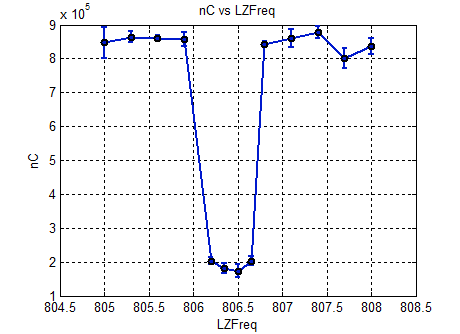
\includegraphics[width=12cm]{landao-zener.png}
  \end{center}
  \caption{Landau-Zener Sweep.}
  \label{exp:landao-zener}
\end{figure}
\begin{figure}
  \begin{center}
    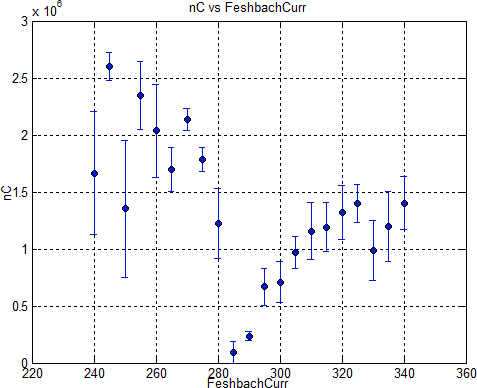
\includegraphics[width=12cm]{feshbach.png}
  \end{center}
  \caption{Feshbach Resonance in $|F=1, m_F=1\rangle$ state.}
  \label{exp:feshbach}
\end{figure}
\begin{figure}
  \begin{center}
    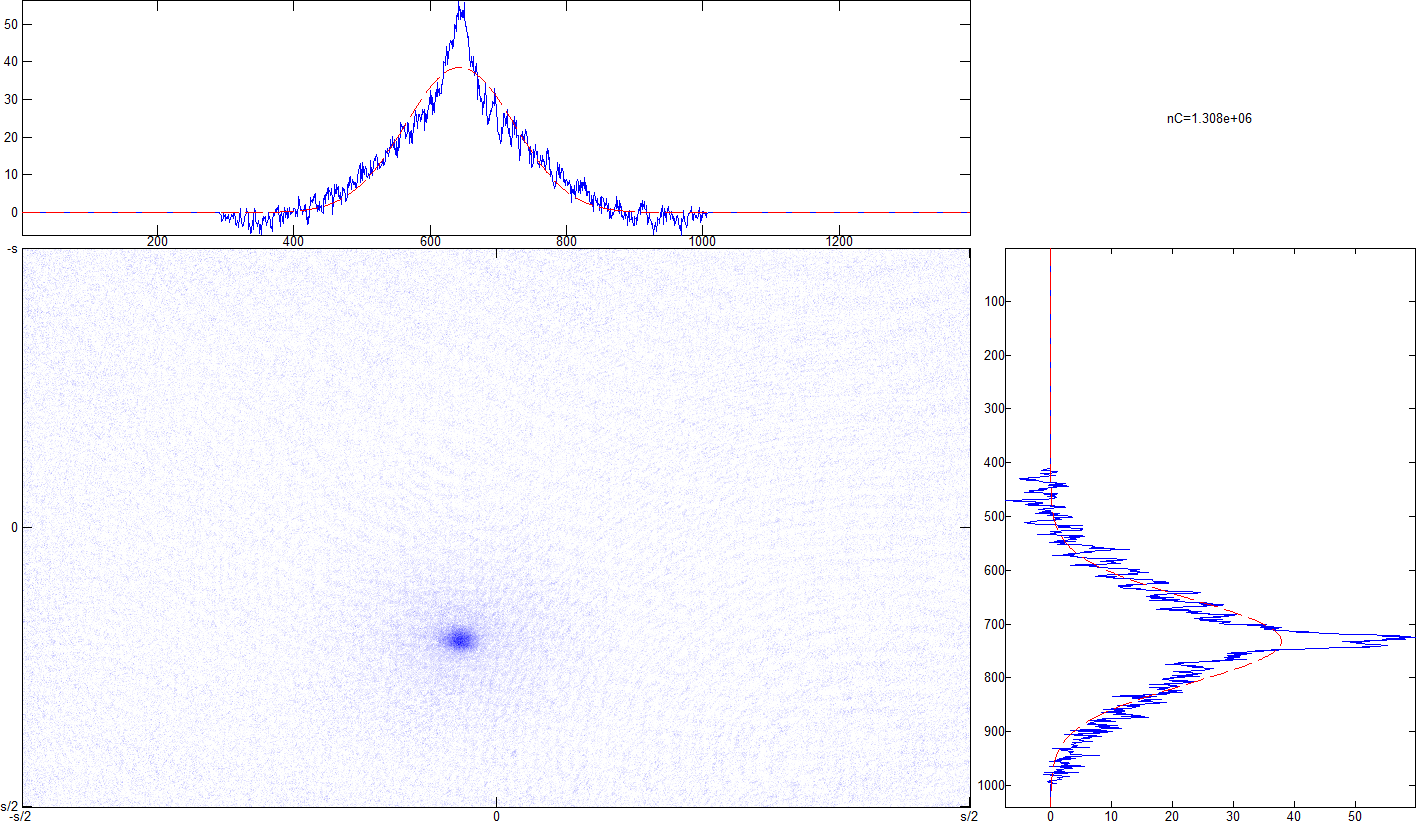
\includegraphics[width=12cm]{bec.png}
  \end{center}
  \caption{BEC with thermal wing.}
  \label{exp:bec-image}
\end{figure}
After evaporation in the magnetic trap, we transfer the atoms into an optical dipole trap (ODT) created with two $15$W $1064$nm laser beams. This transfer need to be adiabatic in order to minimize heating and maximize transfer efficiency. After exploring different transfer schemes, the best method we have found is to turn on the ODT in full power before evaporating in the magnetic trap and ramp down the magnetic trap after evaporation in $200$ms. In this way, we can accumulate $2\cdot10^7$ atoms in the ODT at a temperature of $20\mu K$.\\
\\
We flip the atoms from $|F=2, m_F=2\rangle$ state to $|F=1, m_F=1\rangle$ state using a Landau-Zener sweep with RF frequency. Figure \ref{exp:landao-zener} shows the atom number in $|F=2, m_F=2\rangle$ versus starting frequency of a $1$MHz wide RF scan in a magnetic field about $1.5$G. We hit the resonance around $806.5$MHz and the transfer efficiency is better than $80\%$.\\
\\
The evaporation in the ODT is aided by a Feshbach resonance. We measure the resonance using the increase in three-body loss rate. Figure \ref{exp:feshbach} shows the atom number after a certain hold time in the ODT with different Feshbach field. The resonance occurs at $285$A ($737$Gs). By comparing the resonance point with know data for the scattering length around the resonance, we set the Feshbach field for our evaporation to $\approx701$Gs which corresponds to a reasonably large scattering length ($\approx100a_0$). The evaporation is done by exponentially lower the ODT power, therefore the trapping depth, in each of the ODT beams from $15$W to $1.5$W over $250$ms. The BEC we get after the evaporation has an atom number of $5\cdot10^{6}$ with a temperature $\approx100$nK and condensation fraction $>90\%$. By varying the evaporation parameters, we are able to observe the BEC with different condensation fraction. Figure \ref{exp:bec-image} is an image of a partially condenced BEC with a condensation fraction $\approx15\%$.
